\documentclass[a4paper]{article}
\usepackage{xcolor}
\usepackage{tikz}
\usepackage{hyperref}
\usepackage[T1]{fontenc}
\usepackage[utf8]{inputenc}
\usepackage{DejaVuSansCondensed}
\usepackage{enumitem}
\usepackage{lastpage}

\setlist{topsep=2pt,itemsep=2pt,partopsep=2pt, parsep=2pt}

\renewcommand*\familydefault{\sfdefault} %% Only if the base font of the document is to be sans serif
\usetikzlibrary{calc,positioning,backgrounds}
\definecolor{cvcolorlight}{HTML}{cdebff}
\definecolor{cvcolordark}{HTML}{1a74e2}
\tikzset{
   dot/.style = {
      circle,
      fill,
      minimum size=#1,
      inner sep=0pt,
      outer sep=0pt,
   },
   dot/.default = 6pt
}
\hypersetup{
   hidelinks,
   pdftitle={Michael Allwright},
}

\makeatletter
\pgfkeys{/cventry/.cd,
   left/.code   = {\def\cventry@left{#1}},
   right/.code    = {\def\cventry@right{#1}},
}
\newcommand{\cventry}[1][]{
   \pgfkeys{/cventry/.cd,
      left = {},
      right = {},
   } 
   \pgfqkeys{/cventry}{#1}   
   \node[dot] (bullet) at (cventryoffset) {};
   \node[left=0.5cm of bullet.center,anchor=mid east] (cventrylabel) {\cventry@left};
   \node[right=1.5cm of bullet.center,anchor=mid west, text width = 14cm] (cventrycontent) {\cventry@right};
   % redefine cventryoffset to the next location
   \node (cventryoffset) at ($(cventryoffset.center |- cventrycontent.south) - (0,0.4)$) {};
}

\pgfkeys{/cvsection/.cd,
   label/.code   = {\def\cvsection@label{#1}},
   icon/.code    = {\def\cvsection@icon{#1}},
   entries/.code = {\def\cvsection@entries{#1}},
}
\newcommand{\cvsection}[1][]{
   \pgfkeys{/cvsection/.cd,
      label = {},
      icon  = {},
      entries = {},
   } 
   \pgfqkeys{/cvsection}{#1}
   \node (icon) at (cvsectionoffset) {\includegraphics[height=0.75cm]{icons/\cvsection@icon}};
   \node[right=1.5cm of icon.center,anchor=west] {{\bfseries \LARGE \cvsection@label}};
   \node (cventryoffset) at ($(icon.center) - (0,0.75)$) {};
   \foreach \entry in {\cvsection@entries} {\entry}
   \begin{scope}[on background layer]
      \draw[ultra thick,cvcolordark] (icon.south) -- (bullet.center);
   \end{scope}
}
\makeatother

\begin{document}%
   \pagestyle{empty}%
   \begin{tikzpicture}[remember picture,overlay]
   %background
   \begin{scope}[on background layer]
      \fill[cvcolorlight,anchor=\south]
      (current page.north west) rectangle
      ($(current page.south west) + (5,0)$);
   \end{scope}

   \node[circle, minimum size=4cm, path picture = {
       \node at (path picture bounding box.center){
           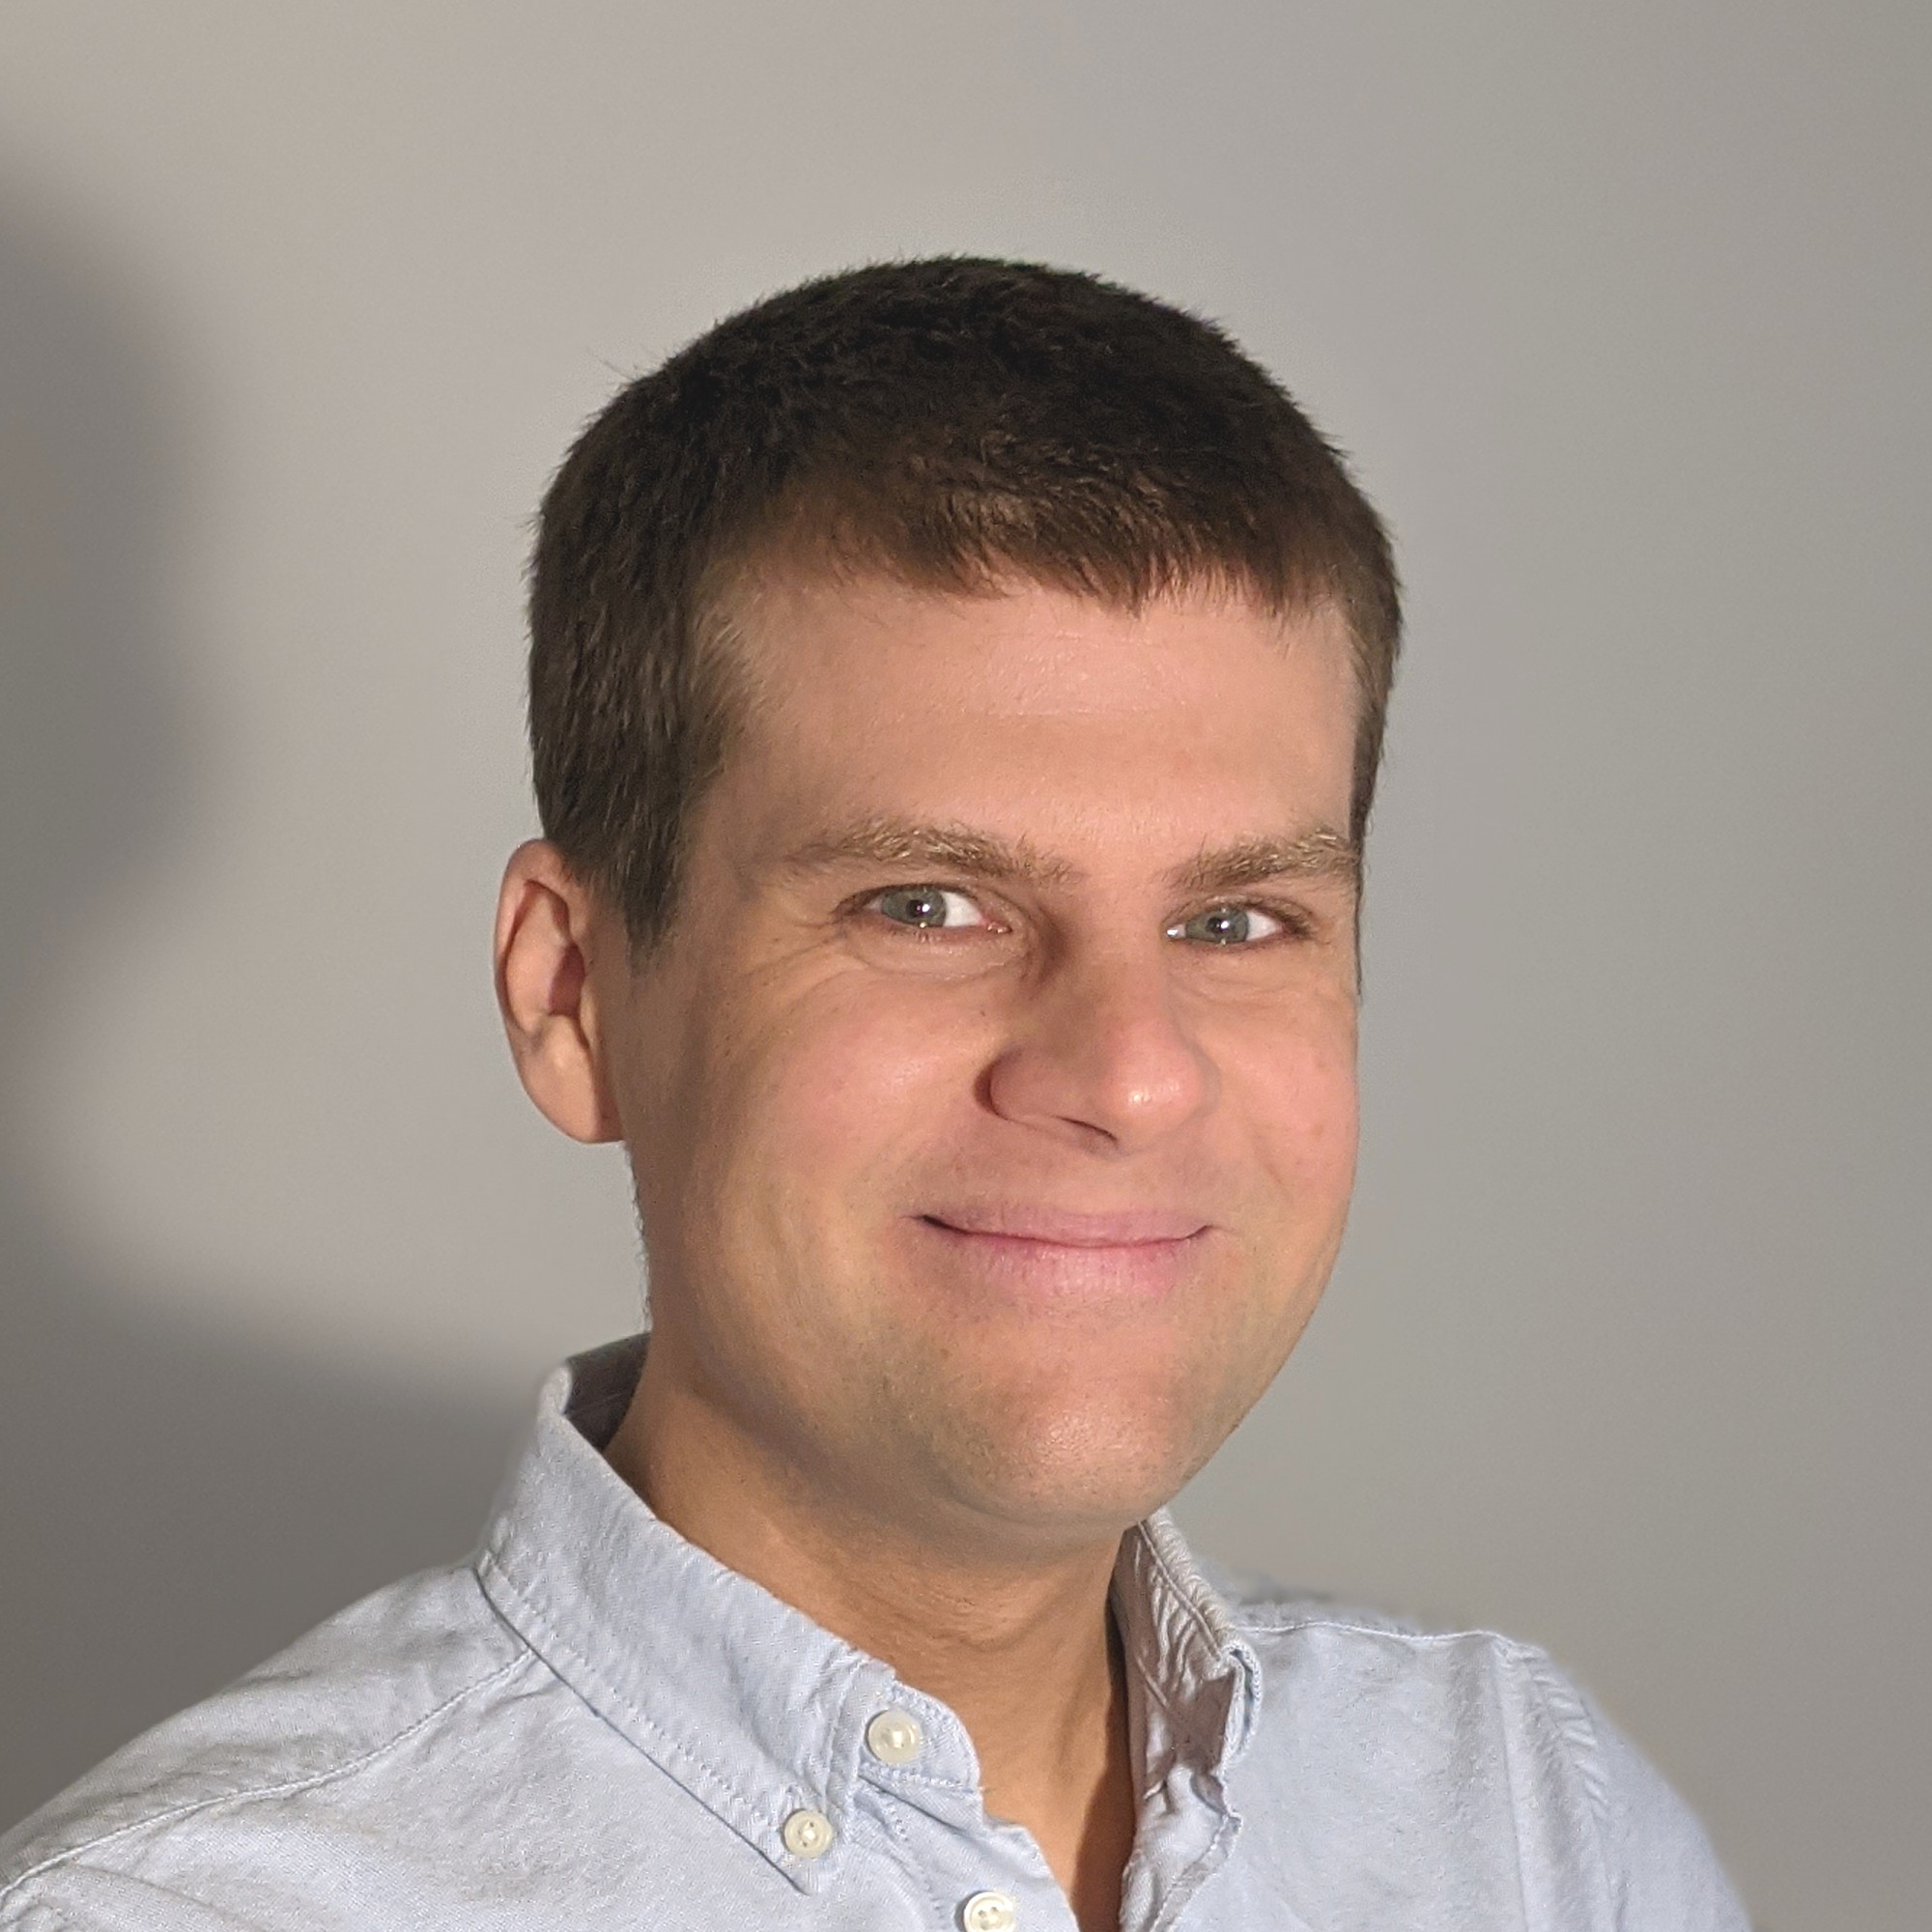
\includegraphics[width=4cm]{profile.jpg}
       };
   }] at (-1,1) {};
   %\fill[cvcolordark] (-1,1) circle [radius=2];

   \node[align=left] at (7.5,1) {
      \textcolor{cvcolordark}{\Huge\bfseries Michael Allwright}\\[0.25cm]%
      \textcolor{cvcolordark}{\LARGE Post-doctoral researcher in robotics}\\[0.25cm]%
      %\textcolor{cvcolordark}{\LARGE Universit\'{e} libre de Bruxelles}\\[0.5cm]%
      \href{tel:+32471731397}{%
         \raisebox{-.25\height}{%
            
\includegraphics[height=0.5cm]{icons/phone}%
         }\hspace{0.125cm}+32\ 471\ 73\ 13\ 97%
      }\hspace{0.6cm}%
      \href{mailto:mallwright@ulb.ac.be}{%
         \raisebox{-.25\height}{%
            
\includegraphics[height=0.5cm]{icons/email}%
         }\hspace{0.125cm}mallwright@ulb.ac.be%
      }\hspace{0.6cm}%
      \href{https://be.linkedin.com/in/mallwright}{%
         \raisebox{-.25\height}{%
            
\includegraphics[height=0.5cm]{icons/linkedin}%
         }\hspace{0.125cm}mallwright%
      }\\[0.125cm]%
      \href{https://orcid.org/0000-0002-0932-3215}{%
         \raisebox{-.25\height}{%
            
\includegraphics[height=0.5cm]{icons/orcid}%
         }\hspace{0.125cm}0000-0002-0932-3215%
      }\hspace{0.6cm}%
      \href{https://github.com/allsey87}{%
         \raisebox{-.25\height}{%
            
\includegraphics[height=0.5cm]{icons/github}%
         }\hspace{0.125cm}allsey87%
      }\hspace{0.6cm}%
      \href{https://allwright.io/}{%
          \raisebox{-.25\height}{%
             
\includegraphics[height=0.5cm]{icons/internet}%
          }\hspace{0.125cm}https://allwright.io/%
      }%
   };
   \node (cvsectionoffset) at (-1,-2.5) {};
   \cvsection[label = {Experience}, icon=work, entries={%
      \cventry[left = {2017 -- now}, right = {
         \textbf{Post-doctoral researcher}
         (Universit\'{e} libre de Bruxelles, Brussels, Belgium)\\
         \begin{itemize}
            \item Studying robotics construction and the formation of centralised control structures in robot swarms
            \item Designing the hardware, electronics, and software for both flying and ground-based robots for studying robotics systems
            \item Contributing significantly to ARGoS, an open-source multi-robot simulator
            \item Establishing and maintaining collaborations between research groups
            %\item Applying for funding and writing project proposals
            %\item Writing conference papers and journal articles
            \item Supervising doctoral and master student projects/theses
         \end{itemize}
      }],
      \cventry[left = {2011 -- 2012}, right = {
         \textbf{Support engineer}
         (Procept, Melbourne, Australia)\\
         \begin{itemize}
            \item Developed software to automate the calibration of mining equipment
            \item Conducted experiments to gain a deeper understanding into the limitations of geological surveying equipment
         \end{itemize}
      }],
      \cventry[left={2010 -- 2011}, right={
         \textbf{Teaching assistant}
         (Swinburne University of Technology, Melbourne, Australia)\\
         \begin{itemize}
            \item Supervised labs and supplemented the lecture material with examples
            \item Explained advanced concepts to students from various topics including: C/C++, assembly, microcontrollers, VHDL, and FPGAs
            %\item Provided feedback through tests and assignments
         \end{itemize}
      }],
   }]
   \node (cvsectionoffset) at ($(cvsectionoffset.center |- cventrycontent.south) - (0,0.75)$) {};
   \cvsection[label={Education}, icon=school, entries={%
      \cventry[left = {2012 -- 2017}, right = {
         \textbf{Doctorate of Natural Sciences}
         (Paderborn University, Paderborn, Germany)\\
         \begin{itemize}
            \item Thesis: \textit{An autonomous multi-robot system for stigmergy-based construction}\\[0.125cm]
            %Examines how stigmergy can be used to coordinate multi-robot construction and presents the design and validation of such a system
            \item Final grade: 1.0 (very good)
            \item Completed a research stay at the Universit\'{e} libre de Bruxelles (ULB) in Belgium to work with the developer of the ARGoS simulator
            \item Completed a research stay at the \'{E}cole polytechnique f\'{e}d\'{e}rale de Lausanne (EPFL) in Switzerland to learn more about the E-puck mobile robot
         \end{itemize}
      }],
      \cventry[left = {2006 -- 2011}, right = {
         \textbf{Bachelor of Engineering}
         (Swinburne University of Technology, Melbourne, Australia)\\
         \begin{itemize}
            \item Finished with first class honours
            \item Completed a semester abroad in Malaysia
            \item Invited to and participated in the Future Leaders Program, an intensive two-week 
            course in Hong Kong, Shanghai and Beijing on conducting business in China
         \end{itemize}
      }],
   }]
   \node (cvsectionoffset) at ($(cvsectionoffset.center |- cventrycontent.south) - (0,0.75)$) {};
   \cvsection[label={Volunteering}, icon=groups, entries={%
      \cventry[left={}, right={Program committee for DARS 2021, ANTS 2020, DARS 2018, ANTS 2018}],
      \cventry[left={}, right={Session chair at ANTS 2020 and ICAR 2017}],
      %\cventry[left={}, right={Answering questions on Stack Overflow and other programming forums}],
   }]
   \node at ($(current page.south east) + (-1.5,1)$) {\small\thepage\hspace{0.025cm}/\hspace{0.025cm}\pageref{LastPage}};
   \end{tikzpicture}
   % PAGE 2
   \newpage%
   \begin{tikzpicture}[remember picture,overlay]
      %background
      \begin{scope}[on background layer]
         \fill[cvcolorlight,anchor=\south]
         (current page.north west) rectangle
         ($(current page.south west) + (5,0)$);
      \end{scope}
      \node (cvsectionoffset) at (-1,3) {};
      \cvsection[label = {Research funding}, icon=money, entries={%
         \cventry[left = {2019 -- 2021}, right = {
            \textbf{Marie Sk\l odowska-Curie Actions: Individual Fellowship}\\
            \begin{itemize}
               \item EUR 166,320 from the European Commision
            \end{itemize}
         }],
         \cventry[left={2018 -- 2019}, right = {
            \textbf{Post-doctoral Research Fellowship}\\
            \begin{itemize}
               \item EUR 42,045 from the Universit\'{e} libre de Bruxelles
            \end{itemize}
         }],
         \cventry[left={2018}, right = {
            \textbf{Endeavour Research Fellowship}\\
            \begin{itemize}
               \item AUD 21,315 from the Australian Department of Education
            \end{itemize}
         }],
      }]
      \node (cvsectionoffset) at ($(cvsectionoffset.center |- cventrycontent.south) - (0,0.75)$) {};
      \cvsection[label={Skills}, icon=build, entries={%
         \cventry[left={}, right={
            \textbf{Software development.}
            Experienced at developing large applications in Rust and C/C++. I frequently also use Python,
            Lua, and Bash for more basic tasks and scripting.
         }],
         \cventry[left={}, right={
            \textbf{Embedded Systems.}
            Competent at designing and manufacturing printed circuit boards (PCBs) in both KiCad and Altium Designer.
            I also have significant experience at writing microcontroller firmware for PCBs and at configuring the
            Linux operating system to support those PCBs.
         }],
         \cventry[left={}, right={
            \textbf{Rapid prototyping.}
            Proficient at designing components for robots in CAD software such as SolidWorks. Experienced at 3D printing and mechanical assembly.
         }],
         %\cventry[left={}, right={
         %   \textbf{Public speaking.}
         %   Confident at public speaking from teaching, giving talks, and taking on roles such as session chair at conferences.}],
         %\cventry[left={}, right={
         %   \textbf{Technical writing.}
         %   Adept at writing conference papers, journal articles, and documentation. I am also proficient at using LaTeX (this CV was created in LaTeX).}],
      }]
      \node (cvsectionoffset) at ($(cvsectionoffset.center |- cventrycontent.south) - (0,0.75)$) {};
      \cvsection[label={Languages}, icon=translate, entries={%
         \cventry[left={}, right={English: Native speaker}],
         \cventry[left={}, right={Dutch: B1 (studying since 2019)}],
         \cventry[left={}, right={German: B1 (studied while completing my doctorate in Germany)}],
         \cventry[left={}, right={French: A2 (studied while living in Brussels)}],
      }]
      \node (cvsectionoffset) at ($(cvsectionoffset.center |- cventrycontent.south) - (0,0.75)$) {};
      \cvsection[label={Interests and hobbies}, icon=gamepad, entries={%
         \cventry[left={}, right={\textbf{Travelling.} I enjoy travelling during my vacations and like to visit different cities and to go hiking in the nature.}],
         \cventry[left={}, right={\textbf{Sport.} I like swimming, running, hiking, and rock climbing.}],
         %\cventry[left={}, right={\textbf{Cooking.} I enjoy cooking, particularly Middle Eastern, Indian, and Asian cuisine.}],
         \cventry[left={}, right={\textbf{Open source.} I am very interested in and supportive of the open-source hardware and software movement. I like to contribute to open-source projects in my spare time.}],
      }]
      \node (cvsectionoffset) at ($(cvsectionoffset.center |- cventrycontent.south) - (0,0.75)$) {};    
      \cvsection[label={Selected Publications}, icon=science, entries={%
         \cventry[left={}, right={Hanqing Zhao, Marco Dorigo, Michael Allwright.
            \textbf{General dynamic neural networks for the adaptive tuning of an omni-directional drive system for reactive swarm robotics.}
            25th International Conference on Methods and Models in Automation and Robotics (IEEE 2021).
            \textcolor{cvcolordark}{\href{https://doi.org/10.1109/mmar49549.2021.9528468}{10.1109/mmar49549.2021.9528468}}
         }],
         %\cventry[left={}, right={Yating Zheng, Michael Allwright, Weixu Zhu, Majd Kassawat, Zhangang Han, Marco Dorigo.
         %   \textbf{Swarm construction coordinated through the building material.}
         %   Communications in Computer and Information Science (Springer 2021).
         %   \textcolor{cvcolordark}{\href{https://doi.org/10.1007/978-3-030-76640-5_12}{10.1007/978-3-030-76640-5\_12}}
         %}],
         %\cventry[left={2020}, right={Yara Khaluf, Michael Allwright, Ilja Rausch, Pieter Simoens, Marco Dorigo.
         %   \textbf{Construction task allocation through the collective perception of a dynamic environment.}
         %   12th International Conference on Swarm Intelligence (Springer 2020).
         %   \textcolor{cvcolordark}{\href{https://doi.org/10.1007/978-3-030-60376-2_7}{10.1007/978-3-030-60376-2\_7}}
         %}],
         \cventry[left={}, right={Weixu Zhu, Michael Allwright, Mary Katherine Heinrich, Sinan O\u{g}uz, Anders Lyhne Christensen, Marco Dorigo.
            \textbf{Formation control of UAVs and mobile robots using self-organized communication topologies.}
            12th International Conference on Swarm Intelligence (Springer 2020).
            \textcolor{cvcolordark}{\href{https://doi.org/10.1007/978-3-030-60376-2_25}{10.1007/978-3-030-60376-2\_25}}
         }],
         %\cventry[left={}, right={Aryo Jamshidpey, Weixu Zhu, Mostafa Wahby, Michael Allwright, Mary Katherine Heinrich, Marco Dorigo.
         %   \textbf{Multi-robot coverage using self-organized networks for central coordination.}
         %   12th International Conference on Swarm Intelligence (Springer 2020).
         %  \textcolor{cvcolordark}{\href{https://doi.org/10.1007/978-3-030-60376-2_17}{10.1007/978-3-030-60376-2\_17}}
         %}],
         \cventry[left={}, right={Michael Allwright, Weixu Zhu, and Marco Dorigo.
            \textbf{An open-source multi-robot construction system.}
            HardwareX (Elsevier 2019).
            \textcolor{cvcolordark}{\href{https://doi.org/10.1016/j.ohx.2018.e00050}{10.1016/j.ohx.2018.e00050}}
         }],
         \cventry[left={}, right={Michael Allwright, Navneet Bhalla, Carlo Pinciroli, Marco Dorigo.
            \textbf{Simulating multi-robot construction in ARGoS.}
            11th International Conference on Swarm Intelligence (Springer 2018).
            \textcolor{cvcolordark}{\href{https://doi.org/10.1007/978-3-030-00533-7_15}{10.1007/978-3-030-00533-7\_15}}
         }],
         \cventry[left={}, right={Michael Allwright, Navneet Bhalla, Marco Dorigo.
            \textbf{Structure and markings as stimuli for autonomous construction.}
            18th International Conference on Advanced Robotics (IEEE 2017).
            \textcolor{cvcolordark}{\href{https://doi.org/10.1109/icar.2017.8023623}{10.1109/icar.2017.8023623}}
         }],
         %\cventry[left={}, right={Michael Allwright, Navneet Bhalla, Haitham El-faham, Anthony Antoun, Carlo Pinciroli, Marco Dorigo.
         %   \textbf{SRoCS: Leveraging stigmergy on a multi-robot construction platform for unknown environments.}
         %   9th International Conference on Swarm Intelligence (Springer 2014).
         %   \textcolor{cvcolordark}{\href{https://doi.org/10.1007/978-3-319-09952-1_14}{10.1007/978-3-319-09952-1\_14}}
         %}],
      }]
      \node at ($(current page.south east) + (-1.5,1)$) {\small\thepage\hspace{0.025cm}/\hspace{0.025cm}\pageref{LastPage}};
   \end{tikzpicture}
\end{document}
